\documentclass[../seminar.tex]{subfiles}

\begin{document}

\subsection{Kubernetes for NFV}
	
\begin{flushleft}
Kubernetes is a relatively new introduction to the NFV world. The network functions that are made to run in a container are referred to as Containerized Network Functions (CNFs). The CNCF (Cloud Native Computing Federation ) is constantly striving to enable Kubernetes as an alternative technology to realize NFV Infrastructure.
\end{flushleft}

\subsection{Kubernetes for Edge}

\begin{flushleft}
The below diagram shows the architecture of Kubeedge project, an initiative to develop Edge platform using Kubernetes.

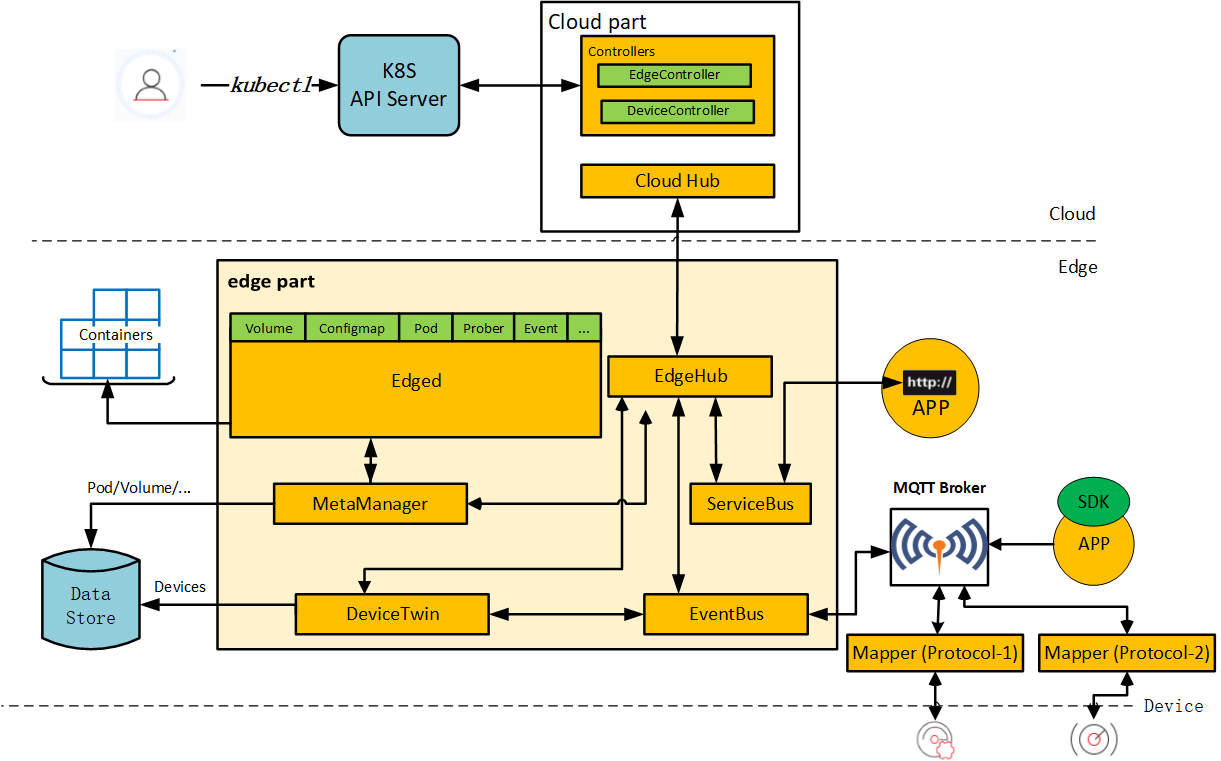
\includegraphics[width=0.9\textwidth]{k8s_edge}
	
\end{flushleft}

\end{document}